\documentclass[12pt, a4paper, twoside]{article}
\usepackage{../labreport}
\usepackage{pdfpages}
\usepackage{circuitikz}

\setlabreportopts[authors={Nandor Kovacs \& Céline Schuster},
    title={Glühlämpchen},
    subtitle={Aufbau von einfachen Schaltkreisen, und die Messung von Strom und Spannung},
    date={\today},
    labdate={24. März 2022}
]

\begin{document}
\maketitlepage
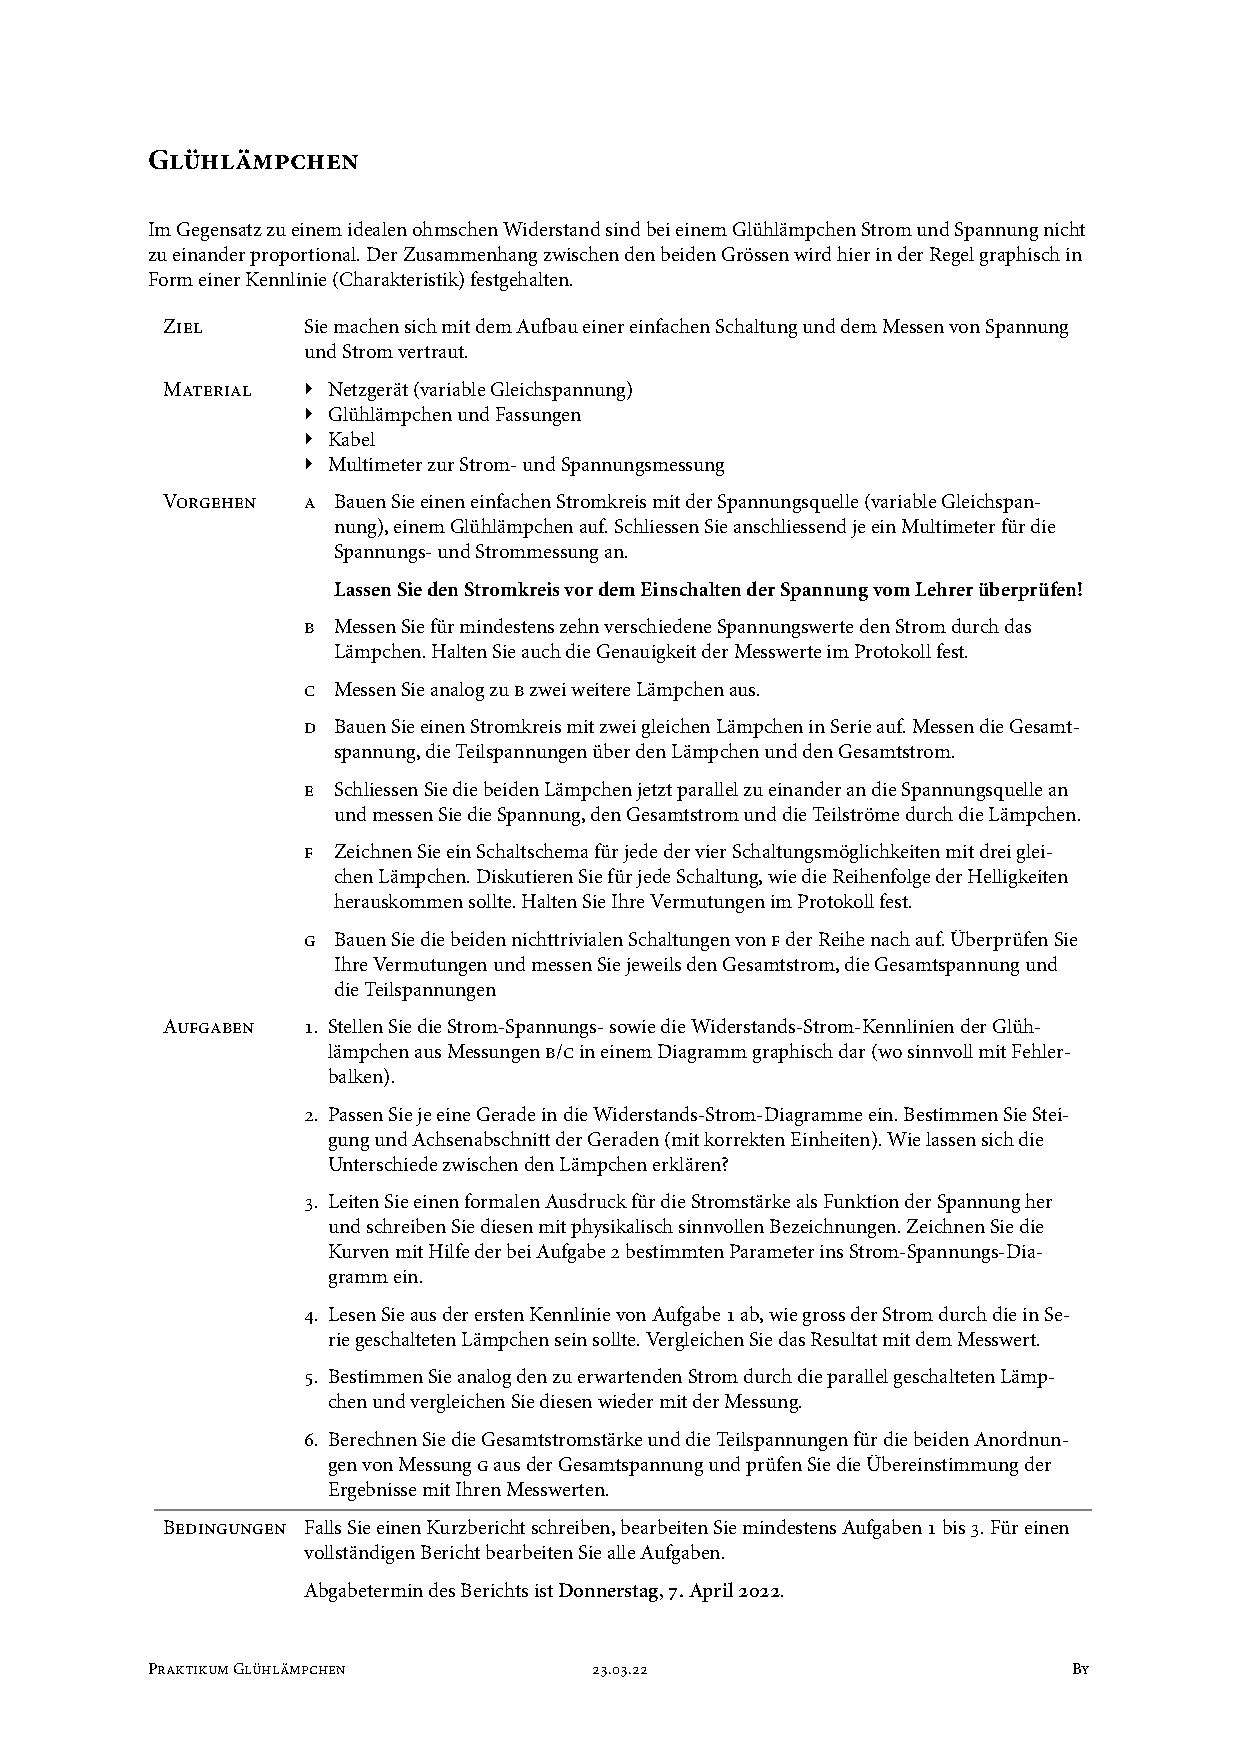
\includepdf[pages={1}]{aufgabenstellung.pdf}
\section{Einleitung}
Im Gegensatz zu konventionellen Widerständen sind Strom und Spannung bei Glühlampen nicht proportional zueinander.
Dennoch stehen diese Größen in einem gewissen Verhältnis zueinander. Wie sie zusammenhängen, ist das Thema dieses Praktikums


\section{Theorie}

\section{Experiment}
Das Experiment bestand aus verschiedenen Stromkreisen, und Messungen an diesen Stromkreisen.
\section{Messungen}
Für dem folgenden Stromkreis haben wir zehn Messungen gemacht.
Bei allen zehn haben wir verschiedene Spannungen angehängt.\\
\begin{align}
  \begin{circuitikz}
    \draw (0, 0.5) to[vsource] (0, 4) to[lamp] (4, 4) to[rmeterwa, t=A, l=$I_{gemessen}$] (4, 0.5) -- (0, 0.5) (0.5, 4) -- (0.5, 5) to[rmeterwa, t=V, l=$U_{gemessen}$] (3.5, 5) -- (3.5, 4);
  \end{circuitikz}
\end{align}

\datatable{c|c|c}{\csvcoli & \csvcolii & \csvcoliii}{Messungen zu der Messgenauigket}{$U_{start}$ & $U_{gemessen}$ & $I_{gemessen}$}{error.csv}{error}




\section{Aufgaben}
\section{Fazit}
\section{Reflektion}
\section{Anhang}
Versuchsanleitung und Originalprotokoll vom \labdate
\end{document}